\documentclass{article}

\usepackage[dvips]{graphicx}
\usepackage{natbib}

\newcommand{\italics}[1]{{\it #1}}

\bibliographystyle{apa}

\begin{document}

\section{Introduction}

\citet{Mills2009} demonstrates the possibility of using statistical classification 
to retrieve continuum values in satellite inverse problems.
A single isoline of a trace substance is retrieved along a
two-dimensional surface.
The potential exists to retrieve multiple isolines and interpolate between
them generating full, two-dimensional fields.
This idea is expanded somewhat in \citet{Mills2011}
which shows that the conditional probabilities make an effective proxy
for the continuum value and that an inverse method derived in this way 
from a maximum likelihood statistical classifier is a robust estimator.
The approach here is more general in that the interpolation
would be performed in the abstract feature space for problems in
which retrievals are not embedded in a real physical space.

This note expands on the work in \citet{Mills2011} by deriving a practical method
of extending statistical classification to continuum inversions and testing it on some example data.
Many nonlinear inverse methods such as nonlinear regression techniques like neural
networks as well as iterative inverse methods such as Levenberg-Marquardt
require minimization of a non-linear function.
Hence the possibility of getting stuck in a local minimum.
The method described here, which is based on a discrete mapping of the Bayesian
classification borders 
does not suffer from this problem since it is not based on minimization.
This \italics{continuum extension of class-borders mapping} also has the advantage
of speed over nonlinear regression methods such as kernel-smoothing which
use all of the training data rather than abstracting it into a more compact model.

\section{Conditional probabilities as a proxy}

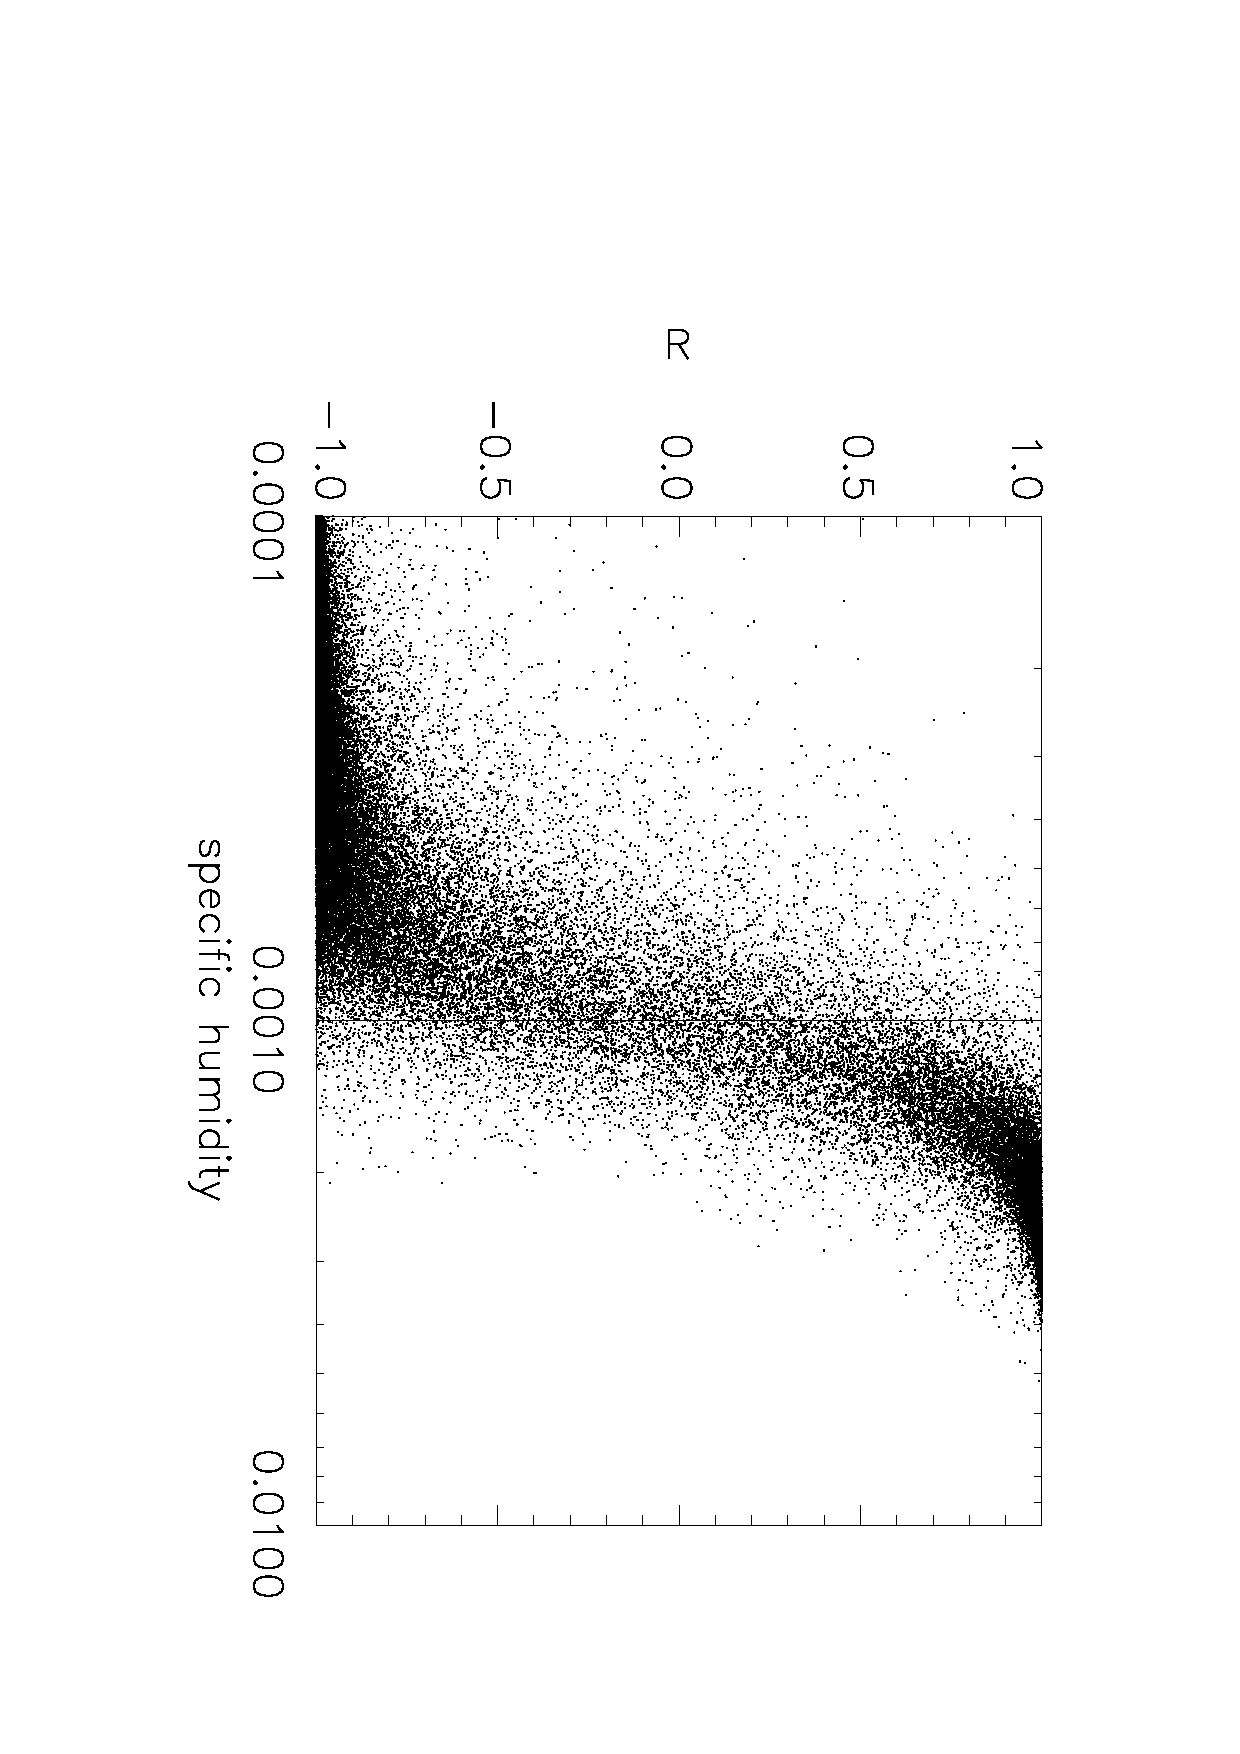
\includegraphics[angle=90,width=0.5\textwidth]{qvsr}

If the statistical classification method returns conditional probabilities,
these can sometimes serve as a good proxy for the continuous quantity.
First, assume that the statistics are Gaussian and write the conditional
probability of the continuous variable:
\begin{equation}
P(y|\vec x) = \frac{1}{\sqrt {2 \pi} \sigma} 
	\left \lbrace \frac{[\bar y(\vec x) - y]^2}{2 \sigma^2} \right \rbrace
\end{equation}
where $\bar y$ is the mean as a function of position in the feature-space,
$\vec x$ and $\sigma$ is the dispersion.

Suppose there are only two classes, with the class division at $y_0$.
Define $R(\vec x)$ as the difference in conditional probabilities:
\begin{eqnarray}
R & = & P(2 | \vec x) - P(1 | \vec x) \\
& = & \int_{y_0}^\infty P(y | \vec x) - \int_{-\infty}^{y_0} P(y|\vec x) \\
& = & \mathrm{erf} \left [ \frac{\bar y(\vec x) - y_0}{\sqrt 2 \sigma} \right ]
\end{eqnarray}
Thus the difference in conditional probabilities is related to the error
function of the mean, $\bar y$, divided by the standard deviation, $\sigma$.

In ``borders classification'', the class of a test point is found by finding
the nearest of a set of border samples and taking the dot product of the
gradient with the displacement vector:
\begin{eqnarray}
j & = & \arg \min_i |\vec b_i - \vec x| \\
p & = & (\vec x - \vec b_j) \cdot \nabla_{\vec x} R |_{\vec x=\vec b_j} 
\label{pdef} \\
c & = & (3+p/|p|)/2
\end{eqnarray}
where $\vec x$ is the test point and $\lbrace \vec b_i \rbrace$ are the border
samples.  
In previous analysis, $R$ was approximated by taking the hyperbolic tangent of
the result at (\ref{pdef}), however from the preceding, it's apparent that the
error function, which is also sigmoid like $\tanh$, 
would be more appropriate:
\begin{equation}
R \approx \mathrm{erf}(p)
\end{equation}
The approximation holds so long as
$\bar y$ is linear in $\vec x$:
\begin{equation}
\bar y(\vec x) \approx y_0 + \sqrt 2 \sigma (\vec x - \vec b_j) \cdot \nabla_{\vec x} R |_{\vec x=\vec b_j}
\end{equation}
If there are multiple class borders, or iso-surfaces, $y_0$, this is not so
hard to enforce as follows below.

This development assumes that the dispersion, $\sigma$, is known,
perhaps through experiment.
We can, however, easily sample two or more iso-surfaces, 
$\lbrace y_0^{(i)} \rbrace$
within the feature space, $\vec x$.  For a given test point, we have:
\begin{equation}
p_i(\vec x) = \frac{\bar y(\vec x) - y_0^{(i)}}{\sqrt 2 \sigma}
\label{baryandp}
\end{equation}
Using two iso-surfaces, 
$i$ and $j$---presumably the closest---we can solve for both
$\sigma$ and $\bar y$:
\begin{eqnarray}
\bar y & = & \frac{p_i y_0^{(j)} - p_j y_0^{(i)}}{p_i - p_j} \\
\sigma & = & \frac{\bar y - y_0^{(i)}}{\sqrt 2 p_i}
\end{eqnarray}
If the surfaces bracket the test point, then it is a simple, linear
interpolation, using $|p|$ as the distance measure. 
Note that in this case, $p_i$ and $p_j$ have opposite sign.
If the surfaces do not
bracket the test point
then $p_i$ and $p_j$ have the same sign and estimates tend to
blow up.

\section{Least squares method}

In most cases we will have multiple realizations of $p$.  We propose the
following least-squares method, weighted by $p$:
\begin{eqnarray}
a_1 & = & - \sqrt 2 \sum_{i=1}^n \frac{1}{p_i} \\
a_2 & = & \sum_{i=1}^n \frac{1}{p_i^2} \\
b_1 & = & - \sqrt 2 \sum_{i=1}^n \frac{y_0^{(i)}}{p_i} \\
b_2 & = & \sum_{i=1}^n \frac{y_0^{(i)}}{p_i^2} \\
d & = & 2 n a_2 - a_1^2 
\end{eqnarray}
\begin{eqnarray}
\bar y & = & (2 n b_2 - a_1 b_1)/d \\
\sigma & = & (a_2 b_1 - a_1 b_2)/d
\end{eqnarray}
Where $n$ is the number of iso-surfaces.  This can be derived by applying the normal equation to (\ref{baryandp}).
While this scheme appears to suffer from two flaws---first, $\bar y$ is being
linearly extrapolated no matter how far the iso-surface, and second,
$\sigma$ is constant---however each item is weighted inversely with the 
value of $p$ which is a measure of distance from the iso-surface.

\bibliography{../agf_bib}

\end{document}

